\documentclass[tikz,border=8pt]{standalone}
\usepackage[utf8]{inputenc}
\usepackage{xcolor}
\usepackage{graphicx}
\usetikzlibrary{arrows.meta,calc,positioning}
\renewcommand{\familydefault}{\sfdefault}

\definecolor{medBlue}   {HTML}{4A86B8}
\definecolor{frozenBlue}{HTML}{8FB8D6}
\definecolor{accentGreen}{HTML}{5DAD6F}
\definecolor{panelGray} {HTML}{CFCFCF}
\definecolor{stackGray} {HTML}{BFBFBF}

\tikzset{
  font=\sffamily,
  arrow/.style={-{Latex[length=2.2mm,width=1.8mm]},draw=black,line width=1.1pt},
  panel/.style={rounded corners=8pt,draw=panelGray,dashed,line width=1.35pt,fill=white},
  model/.style={rectangle,rounded corners=2pt,draw=none,fill=medBlue,text=white,
    minimum width=2.8cm,minimum height=1.4cm,align=center,
    inner xsep=6pt,font=\bfseries\small},
  modelfrozen/.style={rectangle,rounded corners=2pt,
    draw=frozenBlue,dashed,line width=1.2pt,fill=frozenBlue!30,text=black!70,
    minimum width=2.8cm,minimum height=1.4cm,align=center,
    inner xsep=6pt,font=\bfseries\small},
  dimtext/.style={font=\sffamily\scriptsize\itshape,text=black!60,align=center},
}

\newcommand{\imagestack}[3]{%
  \begin{scope}
    \node[rectangle,draw=black,line width=0.6pt,fill=stackGray,
          minimum width=2.2cm,minimum height=2.2cm] at ($#2+(0.22,0.22)$) {};
    \node[rectangle,draw=black,line width=0.6pt,fill=stackGray!70,
          minimum width=2.2cm,minimum height=2.2cm] at ($#2+(0.11,0.11)$) {};
    \node[rectangle,draw=black,line width=0.8pt,
          minimum width=2.2cm,minimum height=2.2cm,
          align=center,inner sep=0pt] (#1) at #2 {#3};
  \end{scope}}

\newcommand{\latentstack}[3]{%
  \begin{scope}
    \node[rectangle,draw=black,line width=0.6pt,fill=stackGray,
          minimum width=1.4cm,minimum height=1.4cm] at ($#2+(0.14,0.14)$) {};
    \node[rectangle,draw=black,line width=0.6pt,fill=stackGray!70,
          minimum width=1.4cm,minimum height=1.4cm] at ($#2+(0.07,0.07)$) {};
    \node[rectangle,draw=black,line width=0.8pt,
          minimum width=1.4cm,minimum height=1.4cm,
          align=center,inner sep=0pt] (#1) at #2 {#3};
  \end{scope}}

\begin{document}
\begin{tikzpicture}[x=1cm,y=1cm]

% ── Panel ────────────────────────────────────────────────
\node[panel,minimum width=18.5cm,minimum height=7.5cm,anchor=north west] at (-.3,7.8){};

% ── Title ────────────────────────────────────────────────
\node[font=\sffamily\bfseries\Large,align=center] at (8.9,7.05)
  {Condition C — MedVAE fine-tuné sur ARCADE (gelé) + tête de segmentation};

% ── Fine-tuning annotation (top) ─────────────────────────
\node[rectangle,rounded corners=3pt,fill=accentGreen!20,draw=accentGreen,
      line width=0.9pt,minimum width=5.5cm,minimum height=0.65cm,
      font=\sffamily\scriptsize,align=center] at (5.2,5.9)
  {Fine-tuné sur ARCADE (reconstruction) puis gelé};

% ── Pipeline ─────────────────────────────────────────────
\imagestack{inp}{(1.5,4.0)}
  {\includegraphics[width=2.2cm,height=2.2cm]{entrée2.png}}

\node[modelfrozen] (enc) at (5.2,4.0)
  {MedVAE\\{\scriptsize encodeur}\\{\scriptsize \textit{gelé — fine-tuné}}};

\latentstack{lat}{(8.5,4.0)}
  {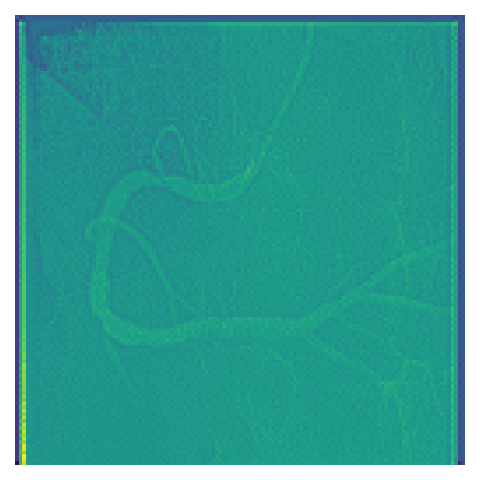
\includegraphics[width=1.4cm,height=1.4cm]{img_latent.png}}

\node[model] (head) at (11.8,4.0)
  {SegHead\\{\scriptsize 2× upsampling ×2}\\{\scriptsize \textit{entraînable}}};

\imagestack{out}{(15.5,4.0)}
  {\includegraphics[width=2.2cm,height=2.2cm]{pred2.png}}

% ── Arrow: fine-tuning annotation to encoder ─────────────
\draw[-{Latex[length=1.8mm,width=1.5mm]},draw=accentGreen,line width=0.9pt]
  (5.2,5.58) -- (5.2,4.8);

% ── Arrows ───────────────────────────────────────────────
\draw[arrow] (inp.east)  -- (enc.west);
\draw[arrow] (enc.east)  -- (lat.west);
\draw[arrow] (lat.east)  -- (head.west);
\draw[arrow] (head.east) -- (out.west);

% ── Dimension labels ─────────────────────────────────────
\node[dimtext] at (1.5,2.5)  {Angiographie X\\512 × 512 — 1 canal};
\node[dimtext] at (8.5,2.5)  {Espace latent\\128 × 128 — 1 canal};
\node[dimtext] at (15.5,2.5) {Masque prédit\\512 × 512 — 26 classes};

\end{tikzpicture}
\end{document}
